\subsection{Interpreter}
\label{interpreter}

\textbf{Scopo}: Comportamentale \\
\textbf{Raggio d'azione}: Oggetti

\paragraph{Definizione} Modello di progettazione che, dato un linguaggio, permette di definire una rappresentazione della sua grammatica insieme a un interprete che utilizza tale rappresentazione per interpretare le frasi in quel linguaggio.

Si definiscono classi di espressioni terminali (elementi di base) e non terminali (combinazioni di elementi), organizzate in una struttura ad albero simile al pattern Composite (\ref{composite}).

\paragraph{Motivazione} Se un particolare tipo di problema si presenta abbastanza frequentemente, allora potrebbe essere utile esprimere le istanze del problema come frasi in un linguaggio semplice, costruendo poi un interprete che risolve il problema interpretando queste frasi. Per esempio, la ricerca di stringhe che corrispondono a un pattern è un problema comune, e le espressioni regolari sono un linguaggio standard per specificare pattern di stringhe: piuttosto che costruire algoritmi personalizzati per far corrispondere ogni pattern alle stringhe, gli algoritmi di ricerca potrebbero interpretare un'espressione regolare che specifica un insieme di stringhe da far corrispondere.

\begin{multicols}{2}
    \begin{figure}[H]
        \centering
        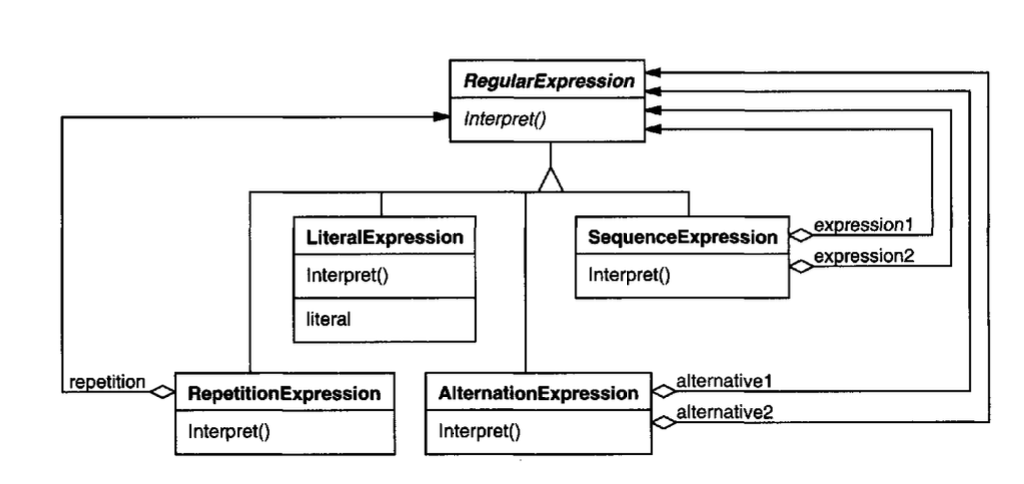
\includegraphics[width=1\linewidth]{assets/pattern/interpreter/interpreter-esempio-class.png}
    \end{figure}
    \columnbreak
    \begin{figure}[H]
        \centering
        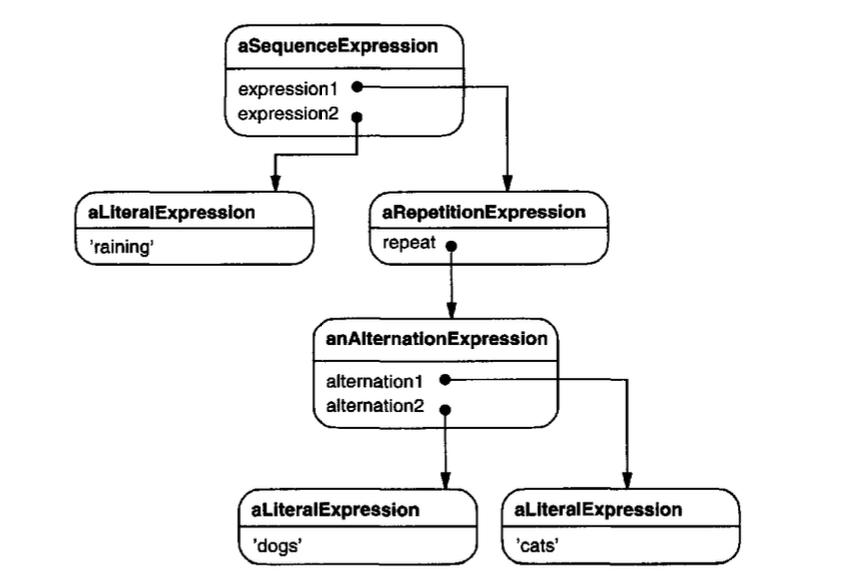
\includegraphics[width=1\linewidth]{assets/pattern/interpreter/interpreter-esempio-object.png}
    \end{figure}
\end{multicols}

Il pattern Interpreter descrive come definire una grammatica per linguaggi semplici, rappresentare frasi nel linguaggio e interpretare queste frasi, usando nel nostro esempio una classe per rappresentare ogni regola grammaticale dove i simboli sul lato destro della regola sono variabili di istanza di queste classi. Ogni espressione regolare definita dalla grammatica è rappresentata da un albero sintattico astratto composto da istanze di queste classi, e possiamo creare un interprete per queste espressioni regolari definendo l'operazione Interpret su ogni sottoclasse che prende come argomento il contesto in cui interpretare l'espressione, contenente la stringa di input e informazioni su quanto di essa è già stata fatta corrispondere. Ogni sottoclasse implementa Interpret per far corrispondere la parte successiva della stringa di input basandosi sul contesto corrente: LiteralExpression controllerà se l'input corrisponde al letterale che definisce, AlternationExpression controllerà se l'input corrisponde a una qualsiasi delle sue alternative, RepetitionExpression controllerà se l'input ha copie multiple dell'espressione che ripete, e così via.

\newpage

\paragraph{Applicabilità} È consigliabile utilizzare il pattern Interpreter quando:
\begin{itemize}
    \item Dato un linguaggio da interpretare, si vogliono rappresentare le sue istruzioni come alberi sintattici astratti;
    \item La grammatica del linguaggio è relativamente semplice;
    \item L'efficienza non è una preoccupazione fondamentale;
\end{itemize}

\begin{figure}[H]
    \centering
    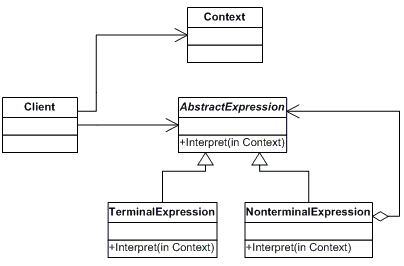
\includegraphics[width=0.75\linewidth]{assets/pattern/interpreter/interpreter-struttura.png}
    \caption{Class Diagram del pattern Interpreter}
\end{figure}

\paragraph{Struttura} Il pattern comprende:
\begin{itemize}
    \item \textbf{AbstractExpression}: Interfaccia o classe astratta che dichiara il metodo \texttt{interpreta}, comune a tutte le espressioni.
    \item \textbf{TerminalExpression}: Classi concrete che rappresentano i simboli di base della grammatica (foglie dell'albero), come numeri o variabili.
    \item \textbf{NonterminalExpression}: Classi concrete che rappresentano combinazioni di espressioni e gestiscono la logica di interpretazione delle sottoespressioni.
    \item \textbf{Context}: contiene informazioni globali per l'interprete.
    \item \textbf{Client}: costruisce (o riceve) un albero sintattico astratto che rappresenta una particolare frase nella lingua definita dalla grammatica. L'albero sintattico astratto è assemblato da istanze delle classi NonterminalExpression e TerminalExpression. Richiama l'operazione \textit{Interpret()}.
\end{itemize}

Le espressioni non terminali coordinano l'interpretazione delle sottoespressioni, aggregando i risultati per ottenere il valore finale dell'espressione.


\paragraph{Conseguenze} Il pattern Interpreter consente quindi di:
\begin{itemize}
    \item Facilitare la modifica ed estensione della grammatica di un dato linguaggio;
    \item Aggiungere nuovi modi per interpretare le espressioni;
\end{itemize}

È bene notare che le grammatiche complesse sono difficili da mantenere.

\newpage
